\chapter{Giới thiệu}

\section{Lý do chọn đề tài}

\subsection{Thách thức từ sự thay đổi sinh học theo thời gian}
Trong những năm gần đây, các hệ thống nhận diện khuôn mặt (Face Recognition - FR) đã đạt được những bước tiến vượt bậc, hoạt động hiệu quả trong các điều kiện tiêu chuẩn với ảnh chụp gần thời điểm xác thực. Tuy nhiên, hiệu năng của các hệ thống này vẫn gặp phải sự suy giảm đáng kể khi đối mặt với các dữ liệu khuôn mặt thay đổi theo thời gian dài hạn.
\\
Về mặt sinh học, khuôn mặt con người là một thực thể thay đổi liên tục. Quá trình lão hóa làm biến đổi cấu trúc xương, cơ và bề mặt da, dẫn đến sự thay đổi của các đặc trưng thị giác cốt lõi. Đây là một thách thức lớn đối với các thuật toán nhận diện, bởi các đặc trưng này cần phải đủ tính "bất biến" (invariant) để nhận diện chính xác qua nhiều năm. Tuy nhiên, thực tế thường xảy ra hiện tượng "trôi đặc trưng" (feature drift), khiến khoảng cách giữa các vector đặc trưng của cùng một người tăng lên theo thời gian, làm giảm độ chính xác của mô hình.
\begin{figure}[H] 
    \centering
    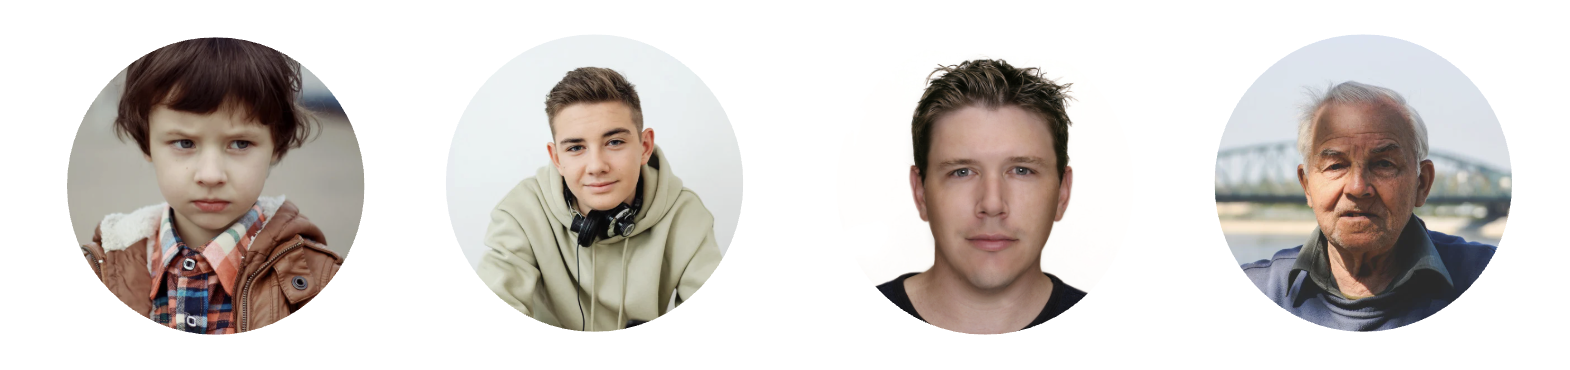
\includegraphics[width=0.8\linewidth]{logos/1.png} 
    \caption{Minh họa sự thay đổi khuôn mặt theo thời gian (Face Aging)} 
\end{figure}

Ngoài ra, sự thiếu hụt các bộ dữ liệu huấn luyện cân bằng, với tỷ lệ ảnh người lớn tuổi thường rất thấp, đặt ra câu hỏi lớn: Liệu sự suy giảm độ chính xác là do giới hạn bản chất của thuật toán hay do sự thiên lệch của dữ liệu? Việc nghiên cứu vấn đề này giúp làm sáng tỏ giới hạn của các mô hình State-of-the-art (SOTA) hiện nay.

\section{Tầm quan trọng của bài toán}

\subsection{Ứng dụng thực tiễn trong An ninh và Xác thực lâu dài}
Tính bền vững theo thời gian (Temporal Robustness) không chỉ là một vấn đề học thuật mà còn là yếu tố sống còn đối với các hệ thống thực tế:
\begin{itemize}
    \item \textbf{Giám sát và An ninh (Surveillance \& Security):} Các hệ thống an ninh cần có khả năng nhận diện các đối tượng truy nã hoặc giám sát ngay cả khi dữ liệu hồ sơ của họ (gallery images) đã được thu thập từ nhiều năm trước.
    \item \textbf{Giấy tờ tùy thân:} Ảnh trên Căn cước công dân (CCCD) hoặc Hộ chiếu (Passport) thường có giá trị sử dụng kéo dài từ 10 đến 20 năm. Các hệ thống e-Gate tại cửa khẩu hoặc xác thực ngân hàng (eKYC) phải xử lý được khoảng cách thời gian lớn (time gap) này mà không gây ra lỗi xác thực sai, đảm bảo trải nghiệm người dùng và an ninh quốc gia.
    \item \textbf{Thiết bị cá nhân:} Với việc mở khóa điện thoại bằng khuôn mặt hàng ngày, hệ thống cần có khả năng "học" và thích nghi với sự lão hóa dần dần của người dùng mà không yêu cầu việc đăng ký lại khuôn mặt liên tục.
\end{itemize}
\begin{figure}[H] 
    \centering
    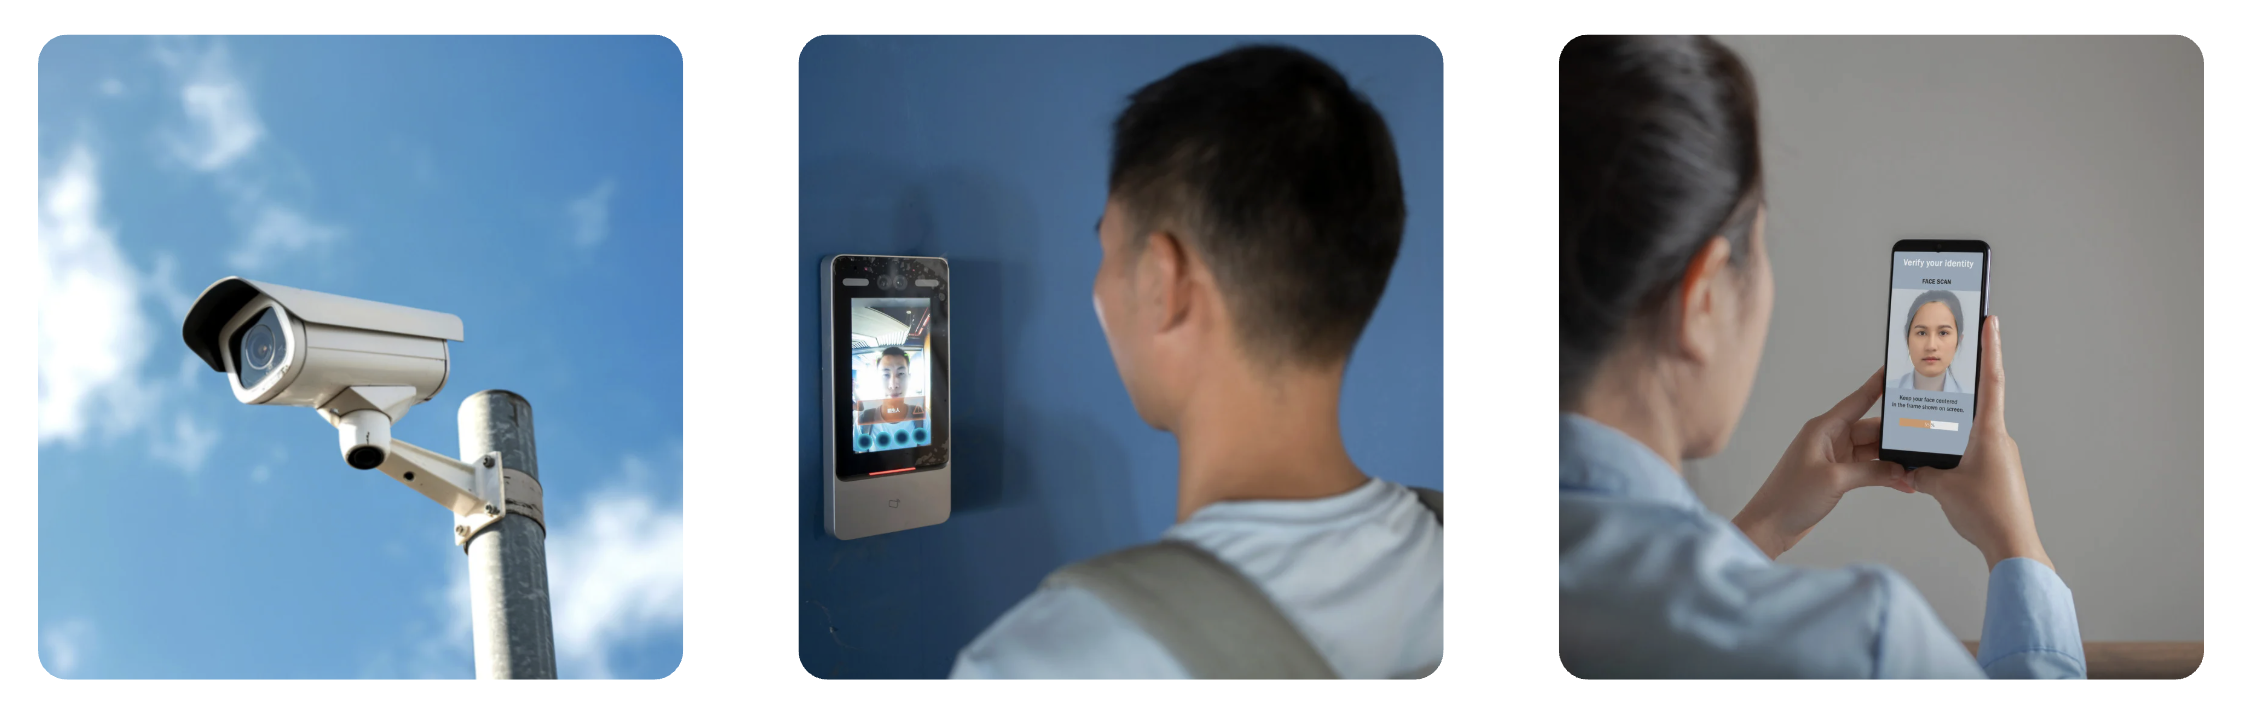
\includegraphics[width=0.8\linewidth]{logos/2.png} 
    \caption{Ứng dụng thực tiễn của nhận diện khuôn mặt bền vững theo thời gian} 
\end{figure}

\subsection{Đóng góp vào việc cải thiện và đánh giá độ tin cậy của thuật toán}
Việc định lượng mức độ suy giảm hiệu năng (degradation rate) của các mô hình tiên tiến như ArcFace hay MagFace theo từng khoảng thời gian (2 năm, 5 năm, 10 năm) mang lại giá trị thực tiễn cao. Nếu hệ thống hoạt động kém trên một nhóm tuổi cụ thể (ví dụ: người cao tuổi), điều này có thể dẫn đến các lỗ hổng bảo mật hoặc sự phân biệt đối xử trong cung cấp dịch vụ số.

Bài toán này tập trung so sánh giữa \textbf{ArcFace} (sử dụng biên góc cố định) và \textbf{MagFace} (sử dụng biên thích ứng dựa trên chất lượng ảnh). Kết quả phân tích các chỉ số như EER hay TAR@FAR sẽ cung cấp cái nhìn sâu sắc (insight) về cách tối ưu hóa hàm loss để xử lý tốt hơn các khuôn mặt có độ tuổi thay đổi, tạo tiền đề cho việc phát triển các mô hình "Age-Invariant" trong tương lai.
